%%%%%%%%%%%%%%%%%%%%%%%%%%%%%%%%%%%%%%%%%%%%%%%%%%%%%%%
% Make sure to add any new macros to the final report 
% to ensure that they do not conflict with existsing
% ones.
%%%%%%%%%%%%%%%%%%%%%%%%%%%%%%%%%%%%%%%%%%%%%%%%%%%%%%%

\section{Introduction}

Consider a basketball player coming the court. They arrive at the three point line and have a decision to make: should they cut to the basket or run to the left corner. Depending on the positions of other players, the state in the game, or whether they are playing at home or away, the player might make a different decision. Scenarios like these produce data generated by complex, nonlinear dynamical systems. Instead of trying to produce the exact equations that lead to dynamics like those described above, we can instead understand these systems by decomposing them into multiple, simpler dynamical systems.

\subsection{Switching Linear Dynamical Systems}

Switching linear dynamical systems(SLDSs) are used to split up complex, nonlinear dynamical system data into a set of linear models. By fitting the data to an SLDS, a nonlinear representation is learned. Given sufficient data and an adequate number of linear models, it can learn the global dynamics of the system.

An SLDS has the following components for each time step $t = 1,2, \dots, T$: a discrete latent state $z_t$, a continuous latent state $x_t$, and an observation $y_t$. The underlying state $z_t$ is in the set $\brac{1,2,\dots,K}$ and is driven by a Markov process:
\[\prob(z_{t+1} = j \mid z_t = i) = \pi_{ij}, \]
where $\brak{\pi_{ij}}_{K\times K}$ is the transition matrix of the process. The underlying continuous state $x_t$ is in $\R^M$ and is driven by conditionally linear dynamics, dependent on the discrete latent state $z_{t+1}$:
\[x_{t+1} = A_{z_{t+1}} x_t + b_{z_{t+1}} + v_t, \]
where $A_k\in\R^{M\times M}$, $b_k\in \R^M$, and $v_t \iid \mathcal{N}(0,Q_{z_{t+1}})$, where $Q_k\in\R^{M\times M}$ is the covariance matrix of the normal distribution. Finally, the observation $y_t$ is generated from the corresponding discrete continuous and discrete latent states:
\[y_t = C_{z_{t}} x_t + d_{z_{t}} + w_t,\]
where $C_k\in\R^{N\times M}$, $d_k\in \R^N$, and $w_t \iid \mathcal{N}(0,S_{z_{t}})$, where $S_k\in\R^{N\times N}$ is the covariance matrix of the normal distribution.

The library of the linear systems involved in the SLDS is denoted by
\[\theta = \brac{\pi_k, A_k, b_k, Q_k, C_k, d_k, S_k \mid k = 1, \dots, K}.\]

\subsection{Fitting SLDSs}

\textcolor{red}{Talk about stick-breaking ... and Polya-gamma ...}

\subsection{Recurrent Switching Linear Dynamical Systems (rSLDSs)}

If a switch in the discrete state of a system should occur when the trajectory enters (or leaves) a particular region, the model will be unable to capture this behavior since the discrete state is a function only of the previous discrete state. To rectify this, we instead consider a recurrent switching linear dynamical system (rSLDS). 

The key difference between an SLDS and an rSLDS is in the update of the  discrete latent state, $z_t$. Instead of depending only on the previous discrete state, the update also depends on the continuous latent variable $x_t$. We can see this difference in dependencies Figure \ref{rSLDS}.

\begin{figure}[h!]
	\centering
	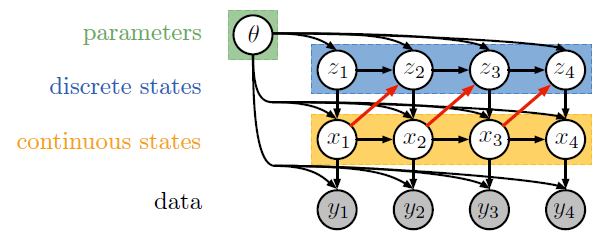
\includegraphics[width=0.5\textwidth]{rSLDS_diagram.png}
	\caption{The black arrows represent the dependencies of a tradidional SLDS, and the red arrows represent the added dependencies of an rSLDS.}
	\label{rSLDS}
\end{figure}

\subsection{Fitting rSLDSs} \textcolor{red}{Differences in fitting SLDS vs rSLDS}

\subsection{Conclusions from the Paper}

In the paper (\textcolor{red}{Cite Linderman Here}), the authors use three examples to demonstrate the capabilities (and limitations) of SLDSs and rSLDSs. These examples are data produced by an actual rSLDS (Synthetic NASCAR), data simulated from a well-studied classical dynamical system (Lorenz Attractor), and real data (Basketball Player Trajectories).

The models performed reasonably well on the synthetic data. Figure \ref{trueNascar} shows the true latent dynamics of the synthetic NASCAR simulation.
\begin{figure}[h!]
	\centering
	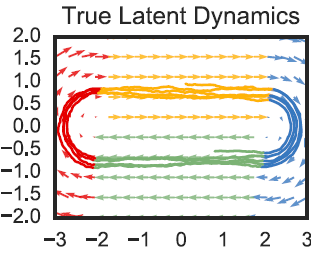
\includegraphics[width=0.35\textwidth]{paper_fig1.png}
	\caption{True dynamics of synthetic NASCAR}
	\label{trueNascar}
\end{figure}

Figure \ref{Nascargen} shows the states generated by both the SLDS and rSLDS fitting of the data. We can see that the rSLDS far outperformed the SLDS. This makes sense because the data was actually generated from an rSLDS, which the SLDS model will not be able to capture. Although this is just simulated data, this proof of concept demonstrates that if the data does indeed come from an SLDS or rSLDS, the approach from the paper will generate a reasonable interpretation of that data.

\begin{figure}[h!]
	\centering
	\begin{subfigure}[b]{0.35\textwidth}
		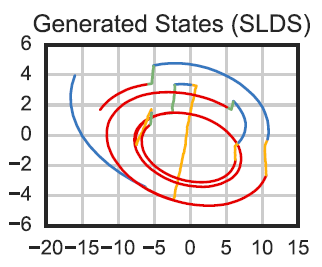
\includegraphics[width=\textwidth]{paper_fig3.png}
		\caption{SLDS}
	\end{subfigure}
	\begin{subfigure}[b]{0.35\textwidth}
		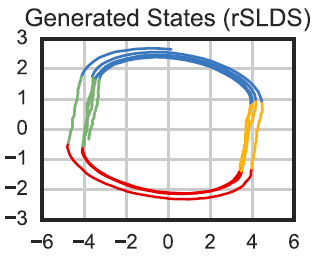
\includegraphics[width=\textwidth]{paper_fig4.png}
		\caption{rSLDS}
	\end{subfigure}
	\caption{Generated states of fit data for synthetic NASCAR}
	\label{Nascargen}
\end{figure}

The next example the authors considered was a system generated by the Lorenz system, a classical nonlinear dynamical system that exhibits chaotic dynamics, switching between two distinct states. However, rather than using Gaussian observations as in a traditional rSLDS, the authors of the paper apply a generalized linear model to the simulated time series data generated by the differential equations and then apply the logistic function. Finally, they collect 100 Bernoulli observations to use as the data to fit the model on.

\begin{figure}[h!]
	\centering
	\begin{subfigure}[b]{0.35\textwidth}
		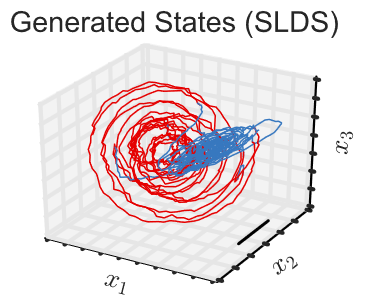
\includegraphics[width=\textwidth]{paper_fig5.png}
		\caption{SLDS}
	\end{subfigure}
	\begin{subfigure}[b]{0.35\textwidth}
		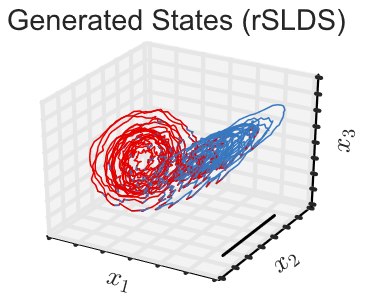
\includegraphics[width=\textwidth]{paper_fig6.png}
		\caption{rSLDS}
	\end{subfigure}
	\caption{Generated states of fit data for the Lorenz data}
	\label{Lorenzgen}
\end{figure}

We can see in Figure \ref{Lorenzgen} that both the SLDS model and the rSLDS model perform reasonably well. The authors found that the rSLDS did perform slightly better than the standard SLDS.

Finally, the authors analyzed data from real basketball players. The data used to fit the model were trajectories from five players in an NBA game between the Miami Heat and the Brooklyn Nets. Rather than an rSLDS, the authors fit the data to a recurrent autoregressive HMM (rAR-HMM), another generalization of the SLDS, where instead of passing through observations of the underlying continuous states, the continuous states are observed directly. These states are assumed to be generated by $K$ latent discrete states. The authors present a subset of these states, and labels them with names of basketball plays that they appear to represent. When comparing these states against those created by a random walk, the predicted states from the recurrent model perform far better; however, there is not evidence that the predicted states capture meaningful patterns in the movements of the players better than the random walk.

\subsection{New Methods}

To reproduce the results of the paper and to apply the models to more systems, we used a more up-to-date approach, as presented in (\textcolor{red}{Cite Blei Paper and Zoltowski paper}). These approaches are Black Box Variational Inference (BBVI) and Laplace Variational EM. These models are called state space models (SSMs).

The first approach is based on variational inference, a method from machine learning that approximates probability densities through optimization. The general idea of this approach is to first propose a family of densities that the target data may arise from and find one that generates data close to the target. The "black box" component of this approach is in reference to a class of these models that avoids any model-specific derivations, so that they can be used for a wide variety of problems. The latter approach combines variational and Laplace approximations over the underlying discrete and continuous variables.

